\documentclass[a4paper,11pt,titlepage]{article}

\usepackage{listings}
\usepackage{amsmath}
\usepackage{amssymb}
\usepackage{amsthm}
\usepackage{graphicx}
\usepackage{hyperref}
\usepackage{parskip}

\setlength{\parindent}{15pt}
\setlength{\emergencystretch}{3em}

\hypersetup{urlcolor=cyan}

\begin{document}

\title{Multi-pose people detection in 3D point clouds}
\author{Stefano Zanella - 621796}
\date{Feb 2017}

\maketitle

\section{Abstract}
This paper describes a people detection algorithm for three-dimensional point
clouds based on the well-known Viola-Jones face recognition algorithm
\cite{violajones}. The key contribution of the project is an implementation of
mentioned algorithm, adapted for work with 3D point clouds. The implementation
consists in a cascaded classifier and its training algorithm. This detector
serves as a cornerstone for the overall people detection algorithm, which
features a variant of the region-growing segmentation algorithm found in the
PCL library. Analysis of the algorithm's performance are provided based on a
given set of 40 images.

\newpage

\section{Introduction}
This paper attempts at extending the current research in the field of
recognition of human beings in three-dimensional point clouds. The key intuition
behind the proposed approach is that human presence in a scene might be
connected to the presence of any part of a human body.

Building a detector flexible enough to recognize any body part (e.g. a face or a
hand), or any sensible combination of them (e.g. a leg and a foot), is a task
that has low chances to lead to good performances. Indeed, also designing a
detector that recognizes bodies in multiple poses is not a simple task, as the
flexibility of human body makes the number of possible poses very high. \\
Moreover, such a detector might not perform well in case of obstructed bodies or
bodies only partially framed into the scene.

Therefore, the proposed approach starts from the most distinguishing part of
a human body: its head. A human head, put in the context of a larger scene,
provides some desirable features:

\begin{itemize}
  \item it's relatively rigid, meaning that it acts approximately as any other rigid
    body that can only be subject to rotation. This is important as it allows to
    be detected by using standard object recognition techniques
  \item it's small compared to the rest of the body, opening the door to algorithms
    that achieve higher performances than those than need to perform larger scans
    of a scene or analyze larger sets of points at a single time
  \item it's possibly the body part that's most discriminative of human nature: e.g.
    it might be hard, at a relative distance, to say if a barefoot belongs to a
    dummy; on the other hand, it's definitely easier to discriminate if a frontal
    head it's human or not. This might be of help to recognition algorithms.
\end{itemize}

The subsequent reasoning step is that, given an accurate way of detecting a
human head in a scene, we can extend the detection to points that seem to
belong to the same object as the head. This is a task that segmentation
algorithms can solve pretty well, with a good range of choices in terms of
speed, accuracy and performances.

This "detection expansion" technique offers a few advantages:

\begin{itemize}
  \item it allows to detect bodies that are partially obstructed or not entirely in
    the scene
  \item it makes the algorithm robust to changes of pose, given the segmentation
    algorithm can correctly identify "compact" objects (i.e. clusters of points
    that are mostly equidistant from each other).
  \item if decomposes a "hard" problem into two problems that have been already well
    treated in literature, and for which a number of efficient solutions exist.
\end{itemize}

As a matter of implementation, two well-known algorithms have been selected:

\begin{itemize}
  \item for head (face) detection, the algorithm devised by Viola and Jones
    \cite{violajones} has been selected and implemented with a number of
    adaptations and improvements made possible by its application in the 3D space
  \item for body detection, a variant of the region-growing segmentation algorithm
    present in the PCL library has been used
\end{itemize}

\subsection*{Overview}
The remaining of this paper will describe more in detail the people detection
algorithm implementation and its peculiarities. We will start by describing the
face detection algorithm and all the specific changes that have been introduced
for it to be applicable to the 3D space. After that the text will focus on the
segmentation algorithm. Finally the results of running the algorithm described
on a validation set of 40 images will be discussed. A selection of ideas for
future improvements closes the paper.

\section{Face detection}
The first step in the processing chain is to detect faces in the current scene.  \\
This is done by employing a boosted cascade detector that takes heavy
inspiration from the work presented by Viola and Jones in their seminal paper.  \\
The detector is composed of a set of rectangular features that get evaluated on
the area currently analyzed, then combining the results in a linear combination
and evaluating the final result against a threshold. \\
Each linear combination of features represents a stage in the final detector: if
an area is recognized as a face in a given stage, the algorithm moves to the
next stage. The algorithm terminates when a stage rejects a sample, or when all
the stages accept it.

\subsection{Features}
A feature is a function over a rectangular area of the sample being analyzed. In
general terms, a feature defines a linear combination that reduces the value of
the pixels in the sample to a single number. More specifically, features can be
of 3 types:

\begin{itemize}
  \item two-rectangle features: they are defined as the difference between the sum of
  the pixels in two rectangular areas. The areas have same size, same shape and
  are horizontally or vertically adjacent
  \item three-rectangle features: in this case what gets computed is the sum of two
  outside rectangles, subtracted from the sum of an inner rectangle of same
  shape and size as the other two
  \item four-rectangle features: the rectangles are positioned in a grid and the
  features computes the difference between the sum of diagonal pairs
\end{itemize}

\begin{figure}[h]
  \centering
  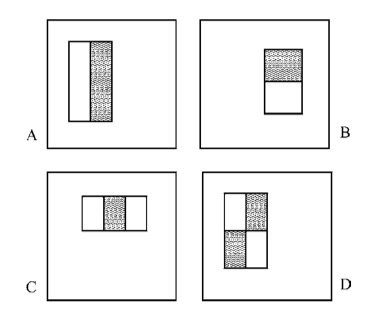
\includegraphics[scale=0.5]{features.jpg}
  \caption{Examples of features relative to the detection window}
  \label{fig:features}
\end{figure}

In order to make the implementation presented in this paper as close as possible
to the original algorithm described by Viola and Jones, features have been
calculated based only on the 2D RGB information of the point cloud. This makes
features calculation very fast and easy to reasonate about as the problem can be
modeled with simple two-dimensional array access. This means the point cloud
passed as input to the detector must be organized.

\subsection{Cascaded classifier}
Evaluation of a single feature is hardly sufficient to obtain a result that can
be distinguished by a random classifier operating over a uniform probability
distribution. A classifier operating with a single feature is named for this
reason \emph{weak classifier}.

Given a detection window $x$, a feature $f$, a threshold $\theta$ and a polarity
$p$, a weak classifier can be described by the equation:

\[ 
  h(x,f,p,\theta) = 
\begin{cases}
  1,& \text{if } pf(x) < p\theta \\ 0,& \text{otherwise}
\end{cases}
\]

To obtain more robust results, weak classifiers can be combined together in a
linear combination. Such a combination is referred to as \emph{strong
classifier}. By means of a strong classifier it's possible to obtain
results that are satisfactory in terms of detection rate and false positive
rate, but at the expense of an increased need for computational power.

The general equation of a strong classifier composed of $T$ weak classifiers is
defined as follows:

\[
  C(X) =
  \begin{cases}
    1& \sum_{t=1}^{T} \log \dfrac{1-\epsilon_{t}}{\epsilon_{t}} h_{t}(X) \geq
    \dfrac{1}{2} \sum_{t=1}^{T} \log \dfrac{1-\epsilon_{t}}{\epsilon_{t}} \\
    0& \text{otherwise}
  \end{cases}
\]

where

\begin{itemize}
  \item $h_{n}(X)$ is the $n$th weak classifier, defined as above
  \item $\epsilon_{n}$ is the weighted error for the $n$th classifier,
    calculated as part of the training process
\end{itemize}

The training process for a strong classifier starts from a set of training
images $(x_{i}, y_{i})$ pre-classified as positive ($y_{i} = 1$) or negative
($y_{i} = 0$), and proceeds as follows:

\begin{itemize}
  \item initialize weights $w_{1,i} = \frac{1}{2m}, \frac{1}{2l}$ for $y_{i} =
    0,1$ respectively, where $m$ and $l$ are the number of negative and positive
    samples
  \item while the false positive rate is above the target level:
    \begin{itemize}
      \item normalize the weights 
        \[
          w_{t,i} \leftarrow \dfrac{w_{t,i}}{\sum_{j=1}^{n} w_{t,j}}
        \]
      \item select the best weak classifier with respect to the weighted error
        \[
          \epsilon_{t} = min_{f,p,\theta} \sum_{i} w_{i} \left|h(x_{i},f, p,
          \theta) - y_{i}\right|
        \]
      \item define
        \[
          h_{t}(x) = h(x, f_{t}, p_{t}, \theta_{t})
        \]
        where $f{t}, p_{t}, \theta_{t}$ are the minimizers of $\epsilon_{t}$
      \item update the weights
        \[
          w_{t+1,i} = w_{t,i}\left(\dfrac{\epsilon_{t}}{1-\epsilon_{t}}\right)^{1-e_{i}}
        \]
        where $e_{i} = 0$ if example $X_{i}$ is classified correctly, $1$
        otherwise
    \end{itemize}
\end{itemize}

This approach would already allow to build a strong classifier that performs
much better than a single weak classifier, but increasing the performance of the
classifier directly impacts computation time.

This can be improved by leveraging a simple idea: in most cases, a detector is
going to reject a sample (i.e. there aren't that many faces in a scene compared
to the overall number of possible samples). So a simple classifier could already
be useful in reducing the number of samples that need to be checked by a more
complex (and thus refined) classifier. \\
This approach is achieved by implementing a variant of AdaBoost \cite{adaboost}
that connect a series of strong classifiers of varying complexity in a chain.
Ideally the detectors should have high detection rate and acceptable false
positive rate. That given, the cascade works as follows: if a sample is
rejected in a stage of the cascade, it won't be processed by later stages. A
sample is declared positive only if all the stages classify it so.

\begin{figure}[h]
  \centering
  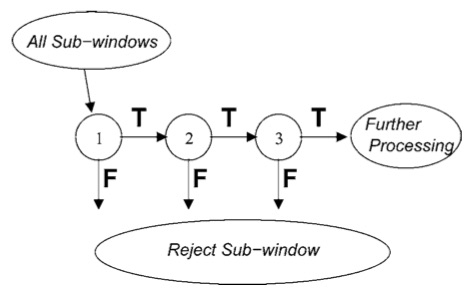
\includegraphics[scale=0.5]{cascade_classifier.jpg}
  \caption{Schematic depiction of a cascade classifier}
  \label{fig:cascade_classifier}
\end{figure}

If we sort the classifiers in order of complexity we would greatly reduce the
average computational power required to classify a sample. Only the actual faces
will require to go through the whole cascade, but the vast majority of the
samples will be rejected early.

The training algorithm for a cascade classifier builds on top of the one for
training a strong classifier. It starts from a fixed target for the maximum
acceptable false positive rate $f$, the overall target false positive rate
$F_{target}$ and for the minimum acceptable detection rate $d$, and proceeds as
follows:

\begin{itemize}
  \item $F_{0} = 1.0, D_{0} = 1.0$
  \item i = 0
  \item while $F_{i} > F_{target}$
    \begin{itemize}
      \item $i++$
      \item create a new stage in the classifier with a strong classifier
      \item while $F_{i} > f \cdot F_{i-1}$
        \begin{itemize}
          \item train a new weak classifier to add to the last strong classifier
          \item evaluate current cascaded classifier on a validation set to
            determine $F_{i}$ and $D_{i}$
          \item while $D_{i} < d$
            \begin{itemize}
              \item decrease threshold of the last trained weak classifier
            \end{itemize}
        \end{itemize}
      \item if $F_{i} > F_{target}$ evaluate current cascaded classifier on set
        of non-face images and replace the current negative set used for
        training with images that are wrongly detected
    \end{itemize}
\end{itemize}

\subsection{Integral image}
For efficient computation of features (both in detection and training), an
integral image representation of the original sample is computed.

In an integral image, each pixel is the sum of all the pixels above and to the
left.

\begin{figure}[h]
  \centering
  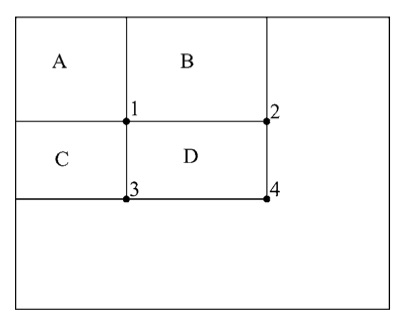
\includegraphics[scale=0.5]{area_sum_integral_image.jpg}
  \caption{The sum of the pixels within rectangle D can be computed with four
  array references: $4+1-2-3$}
  \label{fig:area_sum}
\end{figure}

Using this representation, the value of a rectangle area can be computed by 4
array references as illustrated in the picture above. Computing any of the
features described in the previous paragraph thus requires a constant number of
operations, independent from the size of the feature.

In practical terms, in order to perform all the required operations on an image
efficiently, we need to store both the integral image and the integral image of
the squares, that is the matrix in which each cell contains the square sum of
the cells above and to the left. This is needed in order to calculate the image
variance with $O(1)$ complexity.

Another interesting aspect of the implementation of the integral image is the
different way it is accessed by the training algorithm and the detection
algorithm. For the training algorithm all that's needed is to have an integral
image of the entire sample. A specific feature is calculated only once on the
overall sample. On the contrary, the detection algorithm needs to calculate
features multiple times across the same image. More importantly, image
normalization must happen on the overall sample in case of the training
algorithm, whereas in the detector each of the image portions scanned needs to
be normalized independently from the rest. \\
These two characteristics pose two problems: how to share the code that
calculates the integral image between the two use cases, and how to make image
normalization as efficient as possible.

The first problem has been solved by collecting the integral image and square
integral image calculation code in a common class named \texttt{IntegralImage}.
This class provides facilities to get various calculations for a specific
rectangle of the image held by a class' instance, such as the area sum, mean and
variance.  Taking it from there, then, in order to solve the second problem two
classes have been designed: \texttt{TrainingSample} and \texttt{SubWindow}. A
training sample maps the use case scenario found in training, which boils down
to simple area sum calculation using the whole integral image. A training sample
also stores information useful for the training itself, as for example a flag
saying if the sample contains a face or not (i.e. if it should be classified
positively or not). A sub-window, instead, maps the use case found in the
detector. The main feature is the possibility to calculate a feature on a
portion of the image that gets normalized independently from the rest of the
image.

Image normalization is required to make training and detection as independent as
possible from lighting conditions and general camera exposure. A form of
normalization useful in this case is variance normalization. This transforms the
input so that the end result has a $N(0,1)$ distribution.
Given a pixel value $x$ belonging to an image $X$, its variance-normalized
counterpart can be expressed as:

\[ x_{norm} = \dfrac{x - \overline{x}}{\sigma^{2}} \]

where $\overline{x}$ is the image's mean value, defined as:

\[ \overline{x} = \dfrac{1}{N} \sum X \]

whereas $\sigma^{2}$ is the square variance, defined as:

\[ \sigma^{2} = \overline{x}^{2} - \dfrac{1}{2} \sum X^{2} \]

We can then calculate the linear combination of a set of variance-normalized
pixels by relying on the following equation:

\[ \sum X_{norm} = \dfrac{\sum X}{\sigma^{2}} \]

We need then to solve the problem of how to efficiently calculate the value of a
feature normalized over a portion of the overall image. We do this by allowing a
\texttt{SubWindow} to be repositioned inside the original image. When
repositioning the sub-window, we recalculate the variance over the new image
portion. This is a step that requires $O(1)$ since the integral square image is
stored alongside with the integral image. At this point we can simply apply the
last equation whenever we calculate an area sum.

To make things easier, an instance of \texttt{SubWindow} stores the coordinates
of the image portion being analyzed (in the form of its top-left and
bottom-right corner). When repositioning the sub-window, we also recalculate and
store the variance of the image portion. By repositioning the sub-window instead
of the feature itself, we can achieve a consistent and position-independent
representation of a feature (i.e. the sub-window takes care of translating and
scaling the feature's coordinates).

\subsection{Sizing the features}
The original implementation of the Viola-Jones algorithm is designed to work on
2D images. This mean it doesn't accept any depth information. For this reason,
in the original papepr, the final detector needs to be run at different scales
in each area in order to take into account the fact that faces might be present
in different sizes. \\
In addition to that, a training algorithm has to focus on limited areas of a
specific scene. We'll call these areas \emph{samples}. The size of these samples
is also affected by the distance, and bears a direct linear relationship to the
size of the features. Determination of the size of a sample obeys the same rules
as the determination of a feature's size.

This extra computational step can be avoided if we consider depth information
present in a point cloud. In particular we can start from a reference sample
size, and then scale it based on the position on the Z-axis of the area of the
scene currently analyzed. \\
The reference sample should be big enough to guarantee it fits heads of any
size, but not any bigger. In other words, the reference sample should be as
small as possible without running into the risk of "cutting off" heads that
appear bigger because of camera distortion.

If the reference sample size is expressed for a sample lying on average 1m away
from the camera, then the size of any given sample can then be calculated just
by dividing the reference size by the sample distance.

In practical terms, this poses two problems: the fact that the calculation
happens on pixels and not of real values, and that the depth is not constant
over a specific area. \\
The first problem is simply solved by rounding up the division to the next
integer. Moreover, since once the sample size has been calculated we need to
calculate the precise pixel coordinates of the rectangle to consider, we take
the extra step of rounding up the upper coordinates (i.e. bottom-right corner),
while at the same time we round down the lower coordinates (i.e. top-left
corner). This ensures that even at a big distance we minimize the effect of
rounding by oversizing the sample square.

The problem of the distance not being constant over an area is solved by always
considering the point being analyzed as the center of a rectangle. While this
seems overly simplistic, we also leverage the sequential scanning of the image.
Given that the reference sample is sized so that small variations in the final
sample size don't affect the detector's performance, if at a certain point we
encounter an outlier (either a NaN or a point with a lot of noise in the
distance information), we can just assume that at least one of its neighbors
contains correct information. In other words, in case we encounter outliers, we
can safely assume that the algorithm already classified or will classify the
area correctly when analyzing neighbor points. \\
The only downside of this approach is that in case of area that are overall
noisy (such as peripheral areas in the camera's field of view) the algorithm
might end up skipping classification on large portions of the image. But in that
case, classification is generally difficult anyway given the low SNR.

Another small inefficiency present in the scanning loop due to this
approximation of an area's average distance is the computation that happens at
the boundaries of the scene. Since a specific point is considered the center of
a square when determining the sample size and position, there must be enough
points in all directions so that a full square can be extracted and analyzed. If
the scanning algorithm is working near the image's boundaries, this condition
might not be respected. In this case, the algorithm also skips detection, based
on the assumption that at some point the same algorithm will analyze a close
neighbor whose distance will allow to include all the points discarded up to
that point because the sample would overflow.

The calculation of the size of a feature is performed on a similar basis but
with a caveat: each feature needs to record additional information relative to
the size of the sample that was used when training it. This is necessary because
by introducing information about image depth in the training algorithm, a
specific feature's size loses all meanings when the feature needs to be
rescaled, if the same information is not related to the size of the sample it
was trained with.

In addition to the point above, depth information is also used to minimize the
amount of features generated and evaluated when training the classifier. In the
2D version of the algorithm, all features of all size from 1x1 to the size of
the image must be generated. In the case of a 3D point cloud, we can reduce the
amount of features to those that fit the smallest sample present in the scene.
Features for bigger samples can be upscaled from the smaller ones. This approach
offer two contrasting aspects:

\begin{itemize}
  \item on one side, resolution is lost when upscaling the features (the bigger the
  size differences among samples, the bigger the loss)
  \item on the other side, starting from a set of features for a bigger sample, opens
  the door to the risk of downscaling a feature to the point it goes to a
  sub-pixel level, resulting in a complete loss of informaton during the training
  process.
\end{itemize}

Trials on the designed algorithm showed that the problem introduced by
downsampling features to sub-pixel sizes was jeopardizing the algorithm's
effectiveness, so the first option was selected.

\section{Body segmentation}
Once a face has been identified by the detection algorithm, an attempt is made
to expand the detection and identify the points that belong to the cloud. The
idea is that since we already know some of the points that belong to the
positive classification, we can use a segmentation technique that starts from
those points and tries to include all the points that supposedly belong to the
same object. One such technique is already implemented in the PCL and goes under
the name of region growing.

Region growing is particularly suitable due to the fact that it requires initial
seed points, and he classification algorithm is designed to provide those.

The main idea of the region growing algorithm is to start from a seed point and
put all the points that match a certain definition of neighbor into the same
region set. The curvature of each point is then checked against a certain
predefined threshold: if it's below the limit, then the point is also added to
the set of seeds.

Once the set of seeds have been exhausted, the algorithm considers the
segmentation of the region complete, and moves on by identifying the next seed
and growing the next region. The algorithm completes when all the points have
been assigned to a region.

In the proposed implementation we use a variant of the above algorithm that
also takes into consideration color information, implemented in the
\texttt{pcl::segmentation::RegionGrowingRGB} class. Practically this differs
from the original algorithm in two ways. First, color information is used
instead of normals to identify neighboring points. Second, a merging algorithm
is ran to control over- and under-segmentation. This algorithm attempts first to
merge neighboring clusters depending on their average color difference. Then it
uses a user-defined parameter to merge together neighboring clusters that appear
to be too small.

The advantage of such algorithm is that it usually performs better on people in
terms of precision since a body is not a smooth surface. The merging algorithm
is also useful to merge together body parts that are usually identified
separately (e.g. attaching a hand to an arm covered by a sleeve).

On the other side, this approach has some drawbacks. The main one being its
computational complexity. In theory this problem would be mitigated by the fact
that we provide the algorithm with initial seeds, so we should be able to
exclude building the majority of segments in a scene. In practice though, even
though the implementation found in PCL exposes a method to build a region based
on a seed, this method still performs the full scene segmentation first.

One possible solution to this problem could be to just grow a region based on
the provided seed and to exclude points that don't match the criteria for the
region being grown. The drawback of this is that the step in which adjacent and
similar regions are merged is lost, making the algorithm less robust.

\section{Implementation details}
The effort to realize the algorithm described so far resulted in the
implementation of a number of different applications that support the main
algorithm. In particular, in the accompanying codebase the source code of the
following programs can be found:

\begin{itemize}
  \item a tool to extract faces from a scene. The tool provides a graphical user
    interface that allows the user to move around a square viewport centered
    around the selected point. A point can be selected with \texttt{Shift +
    Click}. The position of the viewport can be adjusted using the arrow keys.
    Pressing \texttt{S} saves the sample to a separate file. The program accepts
    as input a folder whenre to read the scenes from, and one where to save the
    samples to. An example invocation is as follows:

    \begin{verbatim}
    make extract_samples in=dataset/samples out=dataset/positive_frontal
    \end{verbatim}

  \item an application that trains a cascaded face detector given a set of
    positive samples and a scene containing only negative samples. The
    application uses the training procedure described in the preceding
    paragraphs. The output of the training is a YAML file containing the
    parameters that can be used to initialize a trained detector. The
    application can be invoked as follows:

    \begin{verbatim}
    make train positive_set=dataset/positive_frontal \
      negative_sample=negative.pcd
    \end{verbatim}

    The input consists of two arguments: a folder where the positive samples are
    located, and the path to a PCD scene that contains only negative samples.

  \item a sample application that scans a set of scenes for people. The
    application accepts as input a folder containing PCD scenes. Each scene will
    be analyzed sequentially.

    \begin{verbatim}
    make run in=dataset/samples
    \end{verbatim}
\end{itemize}

In addition to this, the codebase contains a set of utilities to facilitate
compilation and execution of the applications in a number of different
environments. Namely:

\begin{itemize}
  \item a \texttt{CMakeLists.txt} file used by CMake to compile all the
    applications described above
  \item a \texttt{Makefile} which provides shortcuts for running the
    applications described above in a virtual environment
  \item a \texttt{Vagrantfile} configuration file and a \texttt{provisioning}
    folder. These are used to set up a Vagrant virtual machine capable of
    compiling and running the applications. Tasks invoked from the
    \texttt{Makefile} automatically bring up the virtual machine if not already
    live
\end{itemize}

The source code of the project is freely available
\href{https://github.com/stefanozanella/people_detection}{on GitHub}.

\section{Results}
Tests on the implementation of the algorithm described so far provided some results that
definitely increase the confidence on the validity of the approach, but overall
performance isn't brilliant. The reason for this is to be found in the limited
size of the training dataset. Also, despite the speed of the face detector, the
speed performance of the segmentation algorithm penalizes the overall time taken
by the algorithm to identify a person.

\subsection{Training dataset}
The training dataset consists in a given set of 40 PCD scenes, one of which
being a negative sample not containing any person. Using this scene as a source
for negatives yields a negative training set of 2392 samples.

\begin{figure}[h]
  \centering
  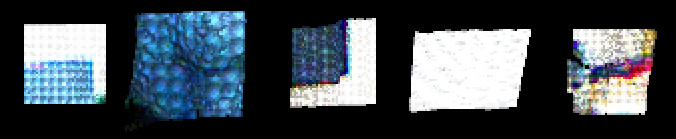
\includegraphics[scale=0.8]{negative_samples.jpg}
  \caption{Example of negative samples used in the training process}
  \label{fig:negative_samples}
\end{figure}

To build the positive training set, instead, the tool described above has been
used. Given the small size of the overall set, heads in all kinds of positions
have been selected. Also, the same head has been used multiple times, by
slightly shifting the selection window around it. With this approach it was
possible to build a positive set of 560 samples.

\begin{figure}[h]
  \centering
  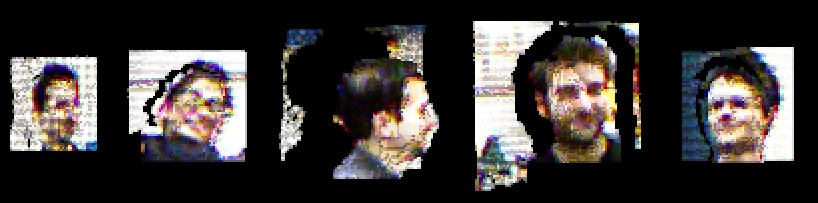
\includegraphics[scale=0.8]{positive_samples.jpg}
  \caption{Example of positive samples used in the training process}
  \label{fig:positive_samples}
\end{figure}

These numbers are barely enough to obtain solid results in training (especially
given that the algorithm is trained to recognize heads in different positions).
As a comparison, in their original paper Viola and Jones used a positive
training set of around 5000 images, and the pool of negative samples had a size
of almost 10000 - out of which a random set of maximum 6000 images was selected
for each trained layer.

In practical terms, this means the algorithm saturates rather quickly and
performances can't be improved beyond a certain point without making the
training algorithm itself unstable. The final consequence of this is that the
final detector has just 3 stages, and in each stage a single detector has been
sufficient to reach the best result possible.

\subsection{Detection performance}
To practically test the validity of the approach, the trained detector has been
applied to the set of samples also used for the training itself. It's important
to note that this is not an optimal approach, as in these cases it's always
recommended to keep the training set and the validation set disjoint to prevent
overfitting of the trained classifier. Nevertheless, given the limited amount of
samples available, the same set has been used both for training and validation.

The results can be analyzed along two distinct dimensions: precision and
accuracy. \\
We can define precision as the algorithm's capability of identifying a person
within a scene, while accuracy deals with how precisely the algorithm identifies
a person's boundaries.

When talking about precision, we can use standard measurements like detection
rate and false positive rate. To go a bit more in depth, we can also analyze
some results and try to carachterize the algorithm's performance in more detail.

In terms of detection rate, the results are highly variable as expected from the
training step. Performance ranges from 0\% to 100\%, with an average of 58.57\%.

\begin{figure}[h]
  \centering
  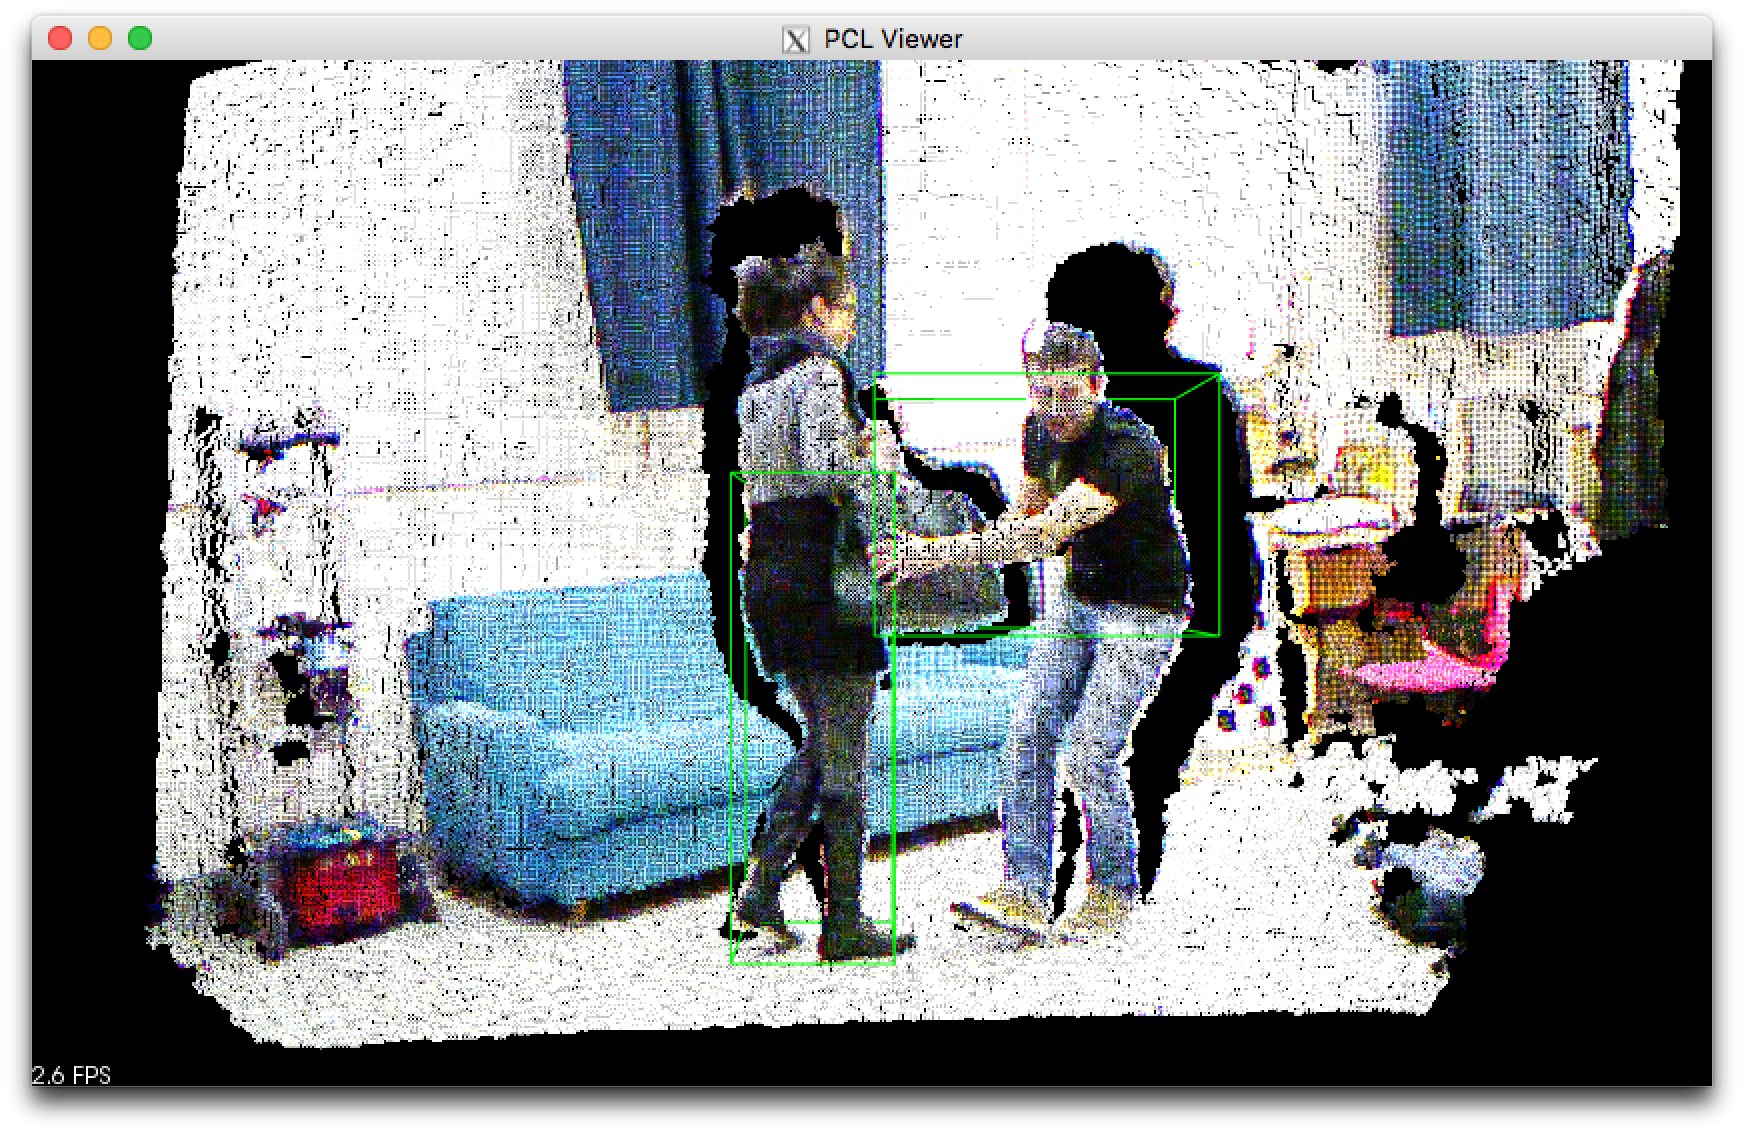
\includegraphics[scale=0.2]{no_missing_but_inaccurate.png}
  \caption{Detection with 100\% detection rate}
  \label{fig:no_missing_but_inaccurate}
\end{figure}

\begin{figure}[h]
  \centering
  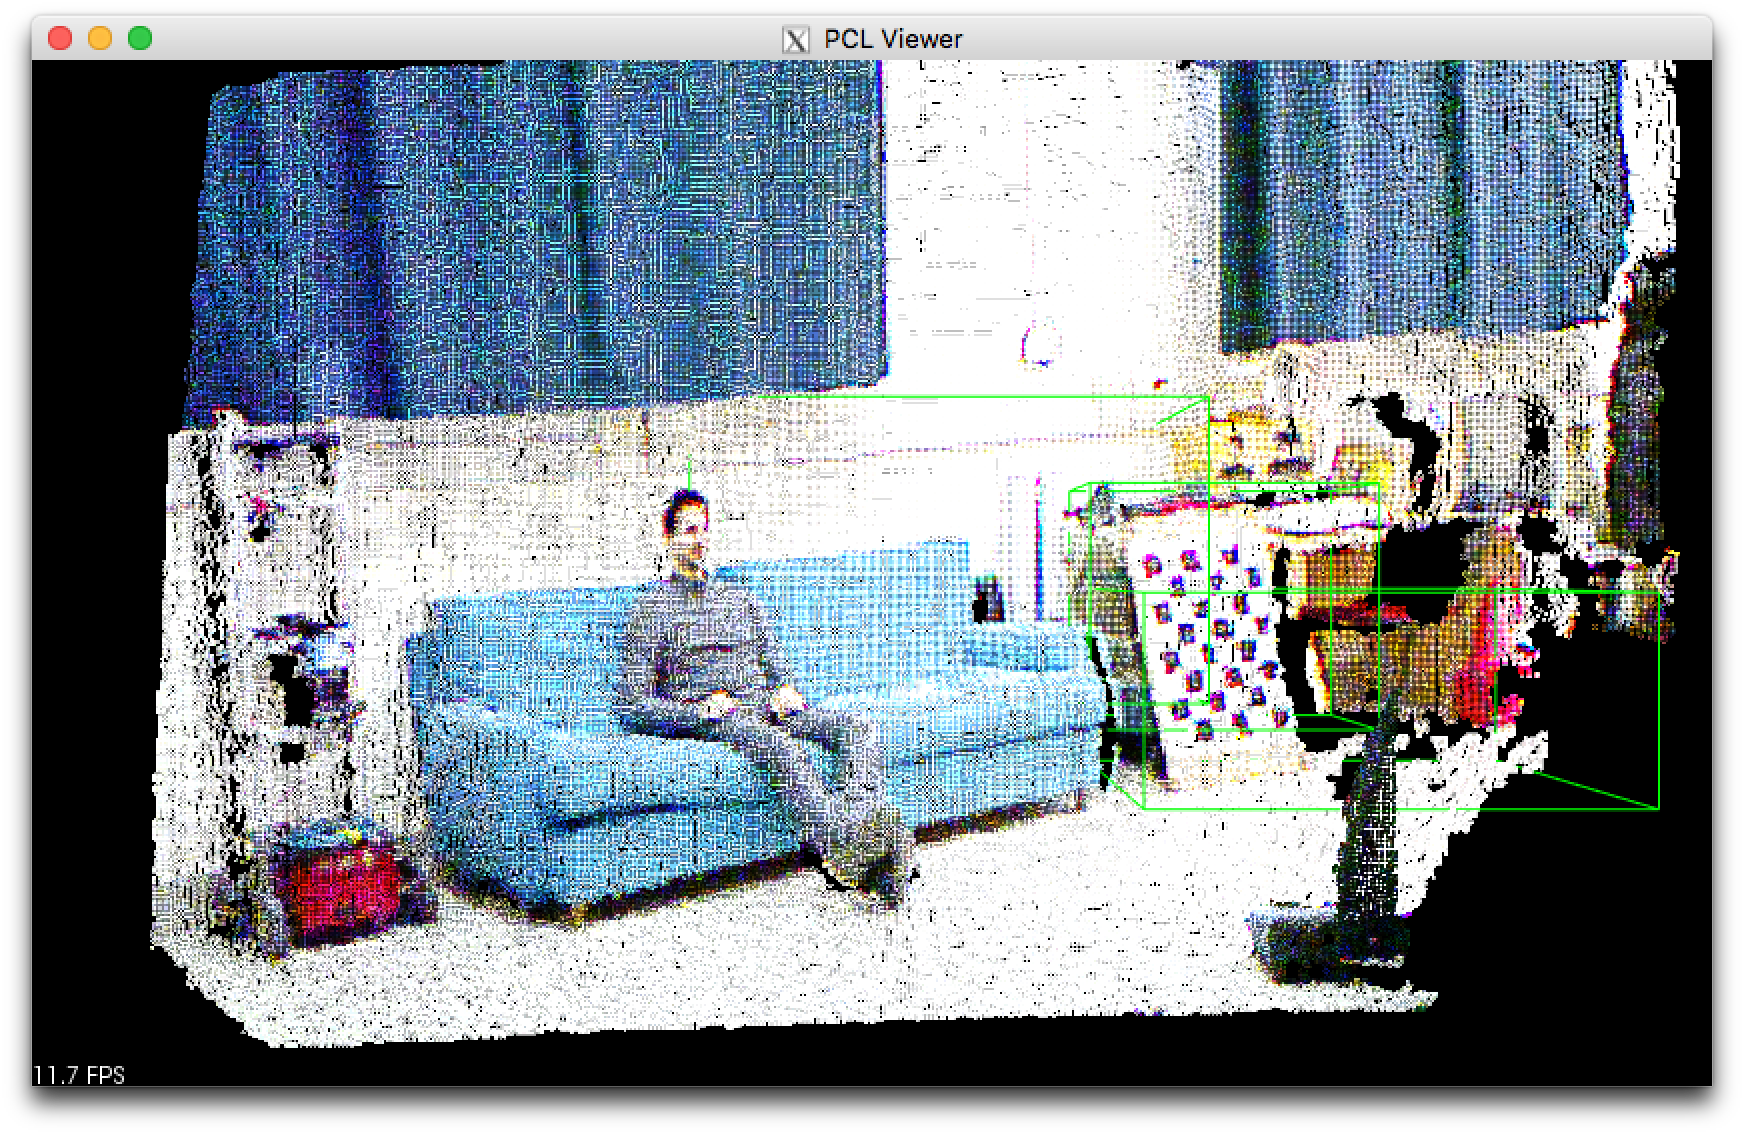
\includegraphics[scale=0.2]{zero_detection_rate.png}
  \caption{Detection with 0\% detection rate}
  \label{fig:zero_detection_rate}
\end{figure}

Figures \ref{fig:no_missing_but_inaccurate} and \ref{fig:zero_detection_rate}
give a visual clue of this variability. In the first case every person in the
scene is correctly detected, while in the second case the only person present is
missed by the algorithm. On average detection on a scene looks more like
figure \ref{fig:one_missing}, where not all the people are correctly identified.

\begin{figure}[h]
  \centering
  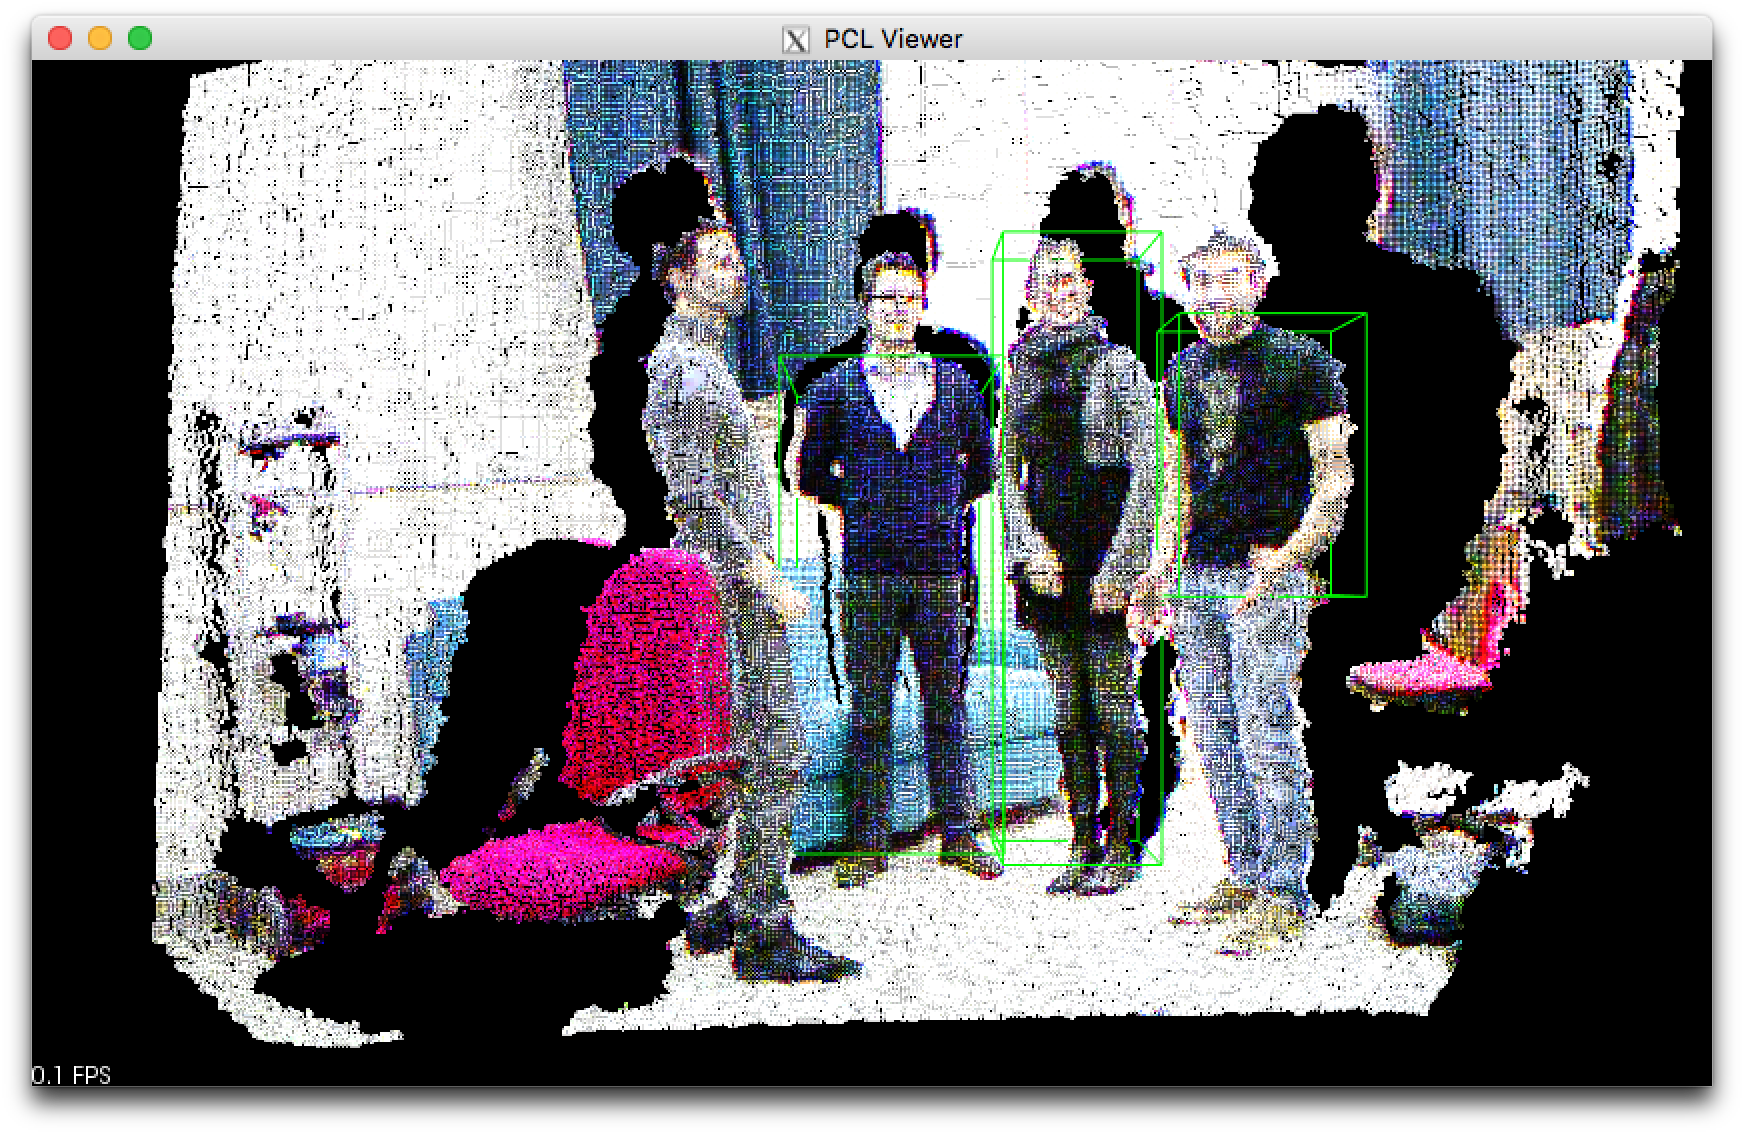
\includegraphics[scale=0.2]{one_missing.png}
  \caption{The algorithm correclty detects only 3 out of 4 people in the scene}
  \label{fig:one_missing}
\end{figure}

Focusing then on the false positive rate, we can see the results are also
variable but a bit more consistent due to the higher amount of negatives present
in a scene. Results vary in a range of 0\% to 0.06\%. Visually, this translates
to a few different patterns. A significant example is the output of the
detection on the scene containing no positives (fig. \ref{fig:false_positives}).
While the algorithm rejects most of the samples, it still identifies a person in
three of the almost 9600 subwindows.

\begin{figure}[h]
  \centering
  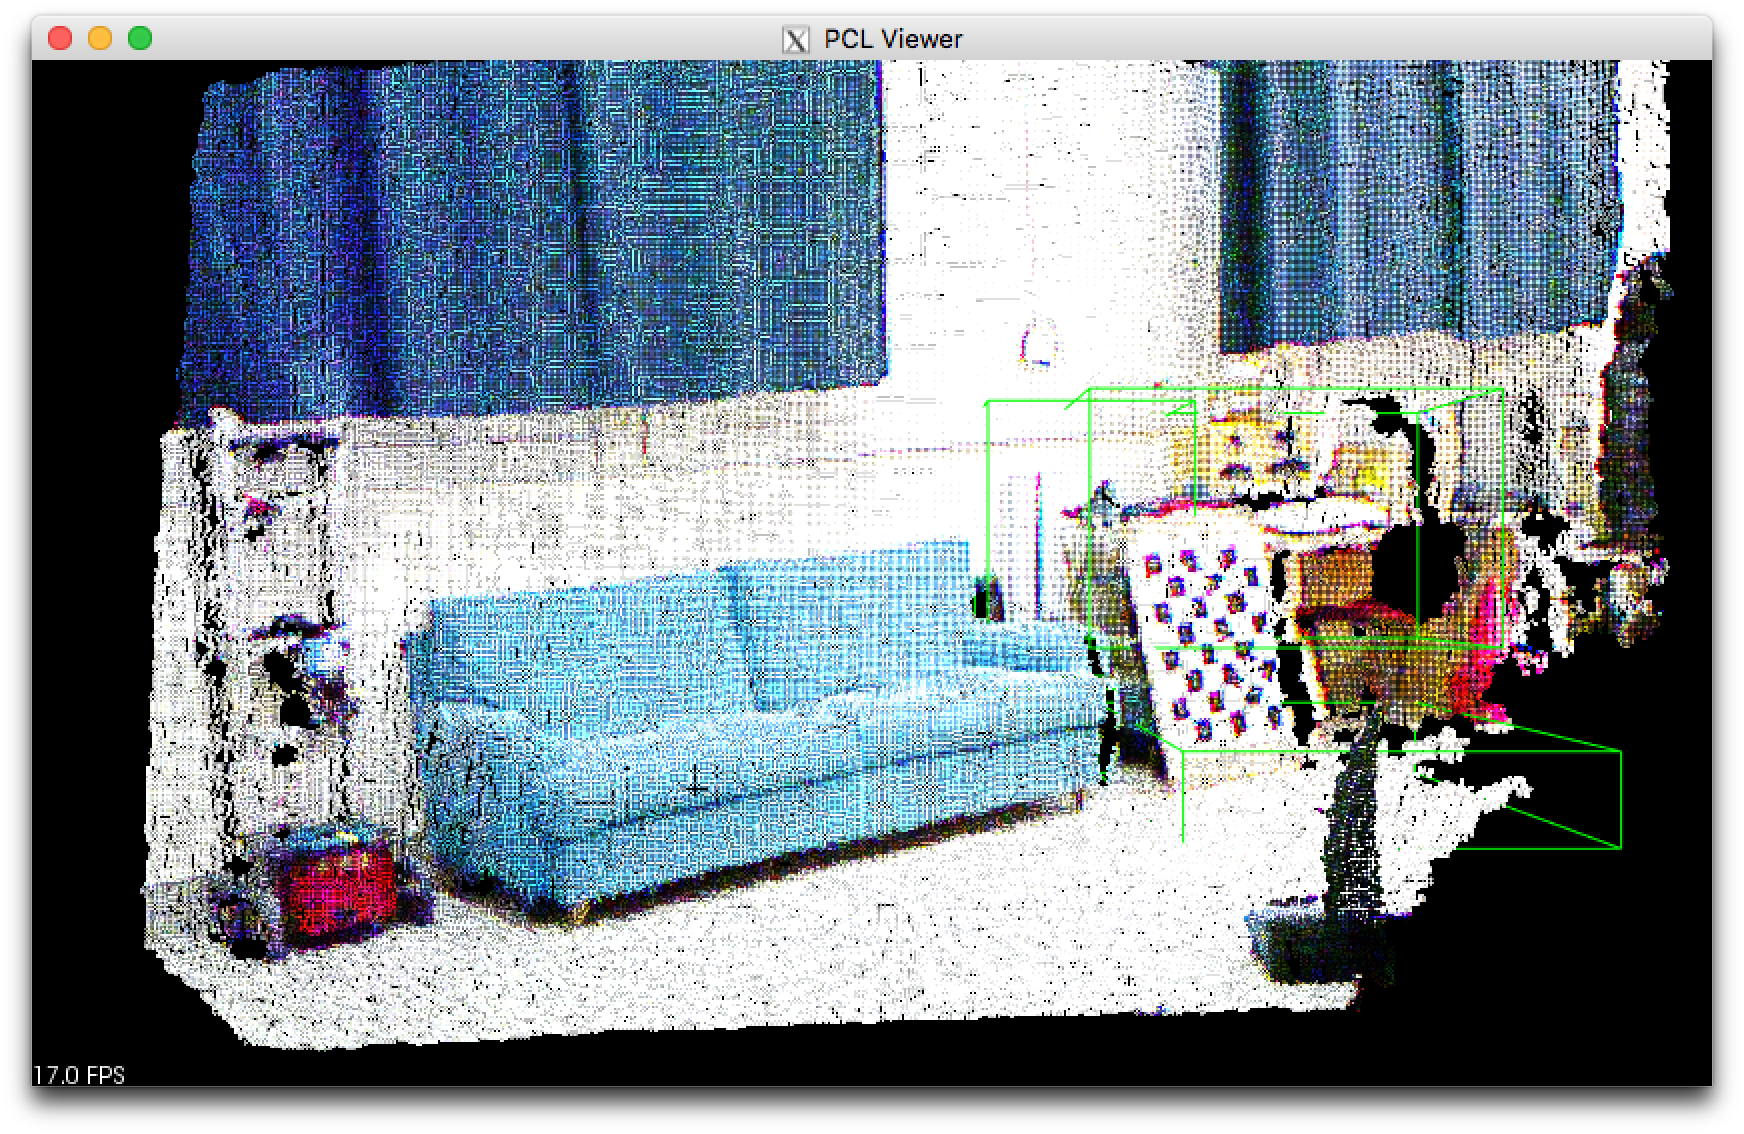
\includegraphics[scale=0.2]{false_positives.png}
  \caption{The algorithm correclty detects only 3 out of 4 people in the scene}
  \label{fig:false_positives}
\end{figure}

Another possible case is the one depicted in figure
\ref{fig:mixed_true_false_positives} where along with a true positive, a
false positive is detected in the chair.

\begin{figure}[h]
  \centering
  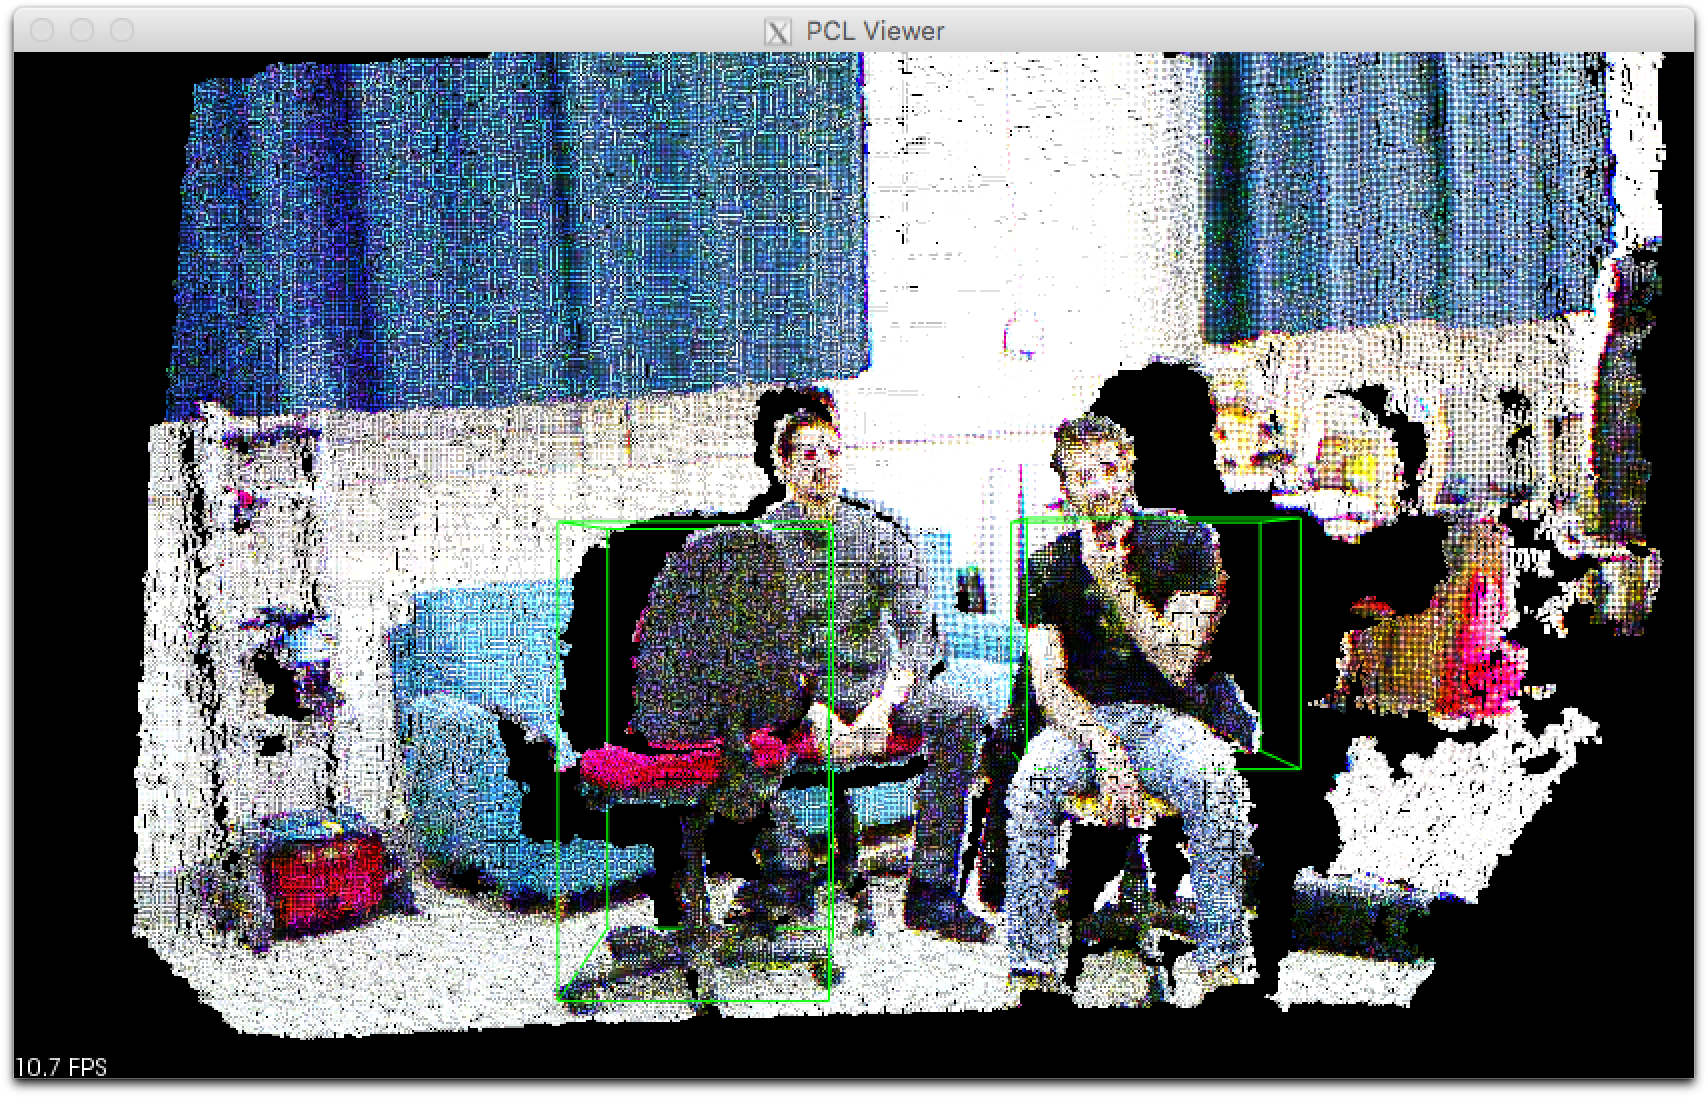
\includegraphics[scale=0.2]{mixed_true_false_positives.png}
  \caption{A true detection is missed and a false positive is detected instead}
  \label{fig:mixed_true_false_positives}
\end{figure}

The numbers given so far only considered a detection as either correct or
incorrect depending on whether mentioned detection was including part of a
person or not. What remains to be analyzed is the accuracy of those detection,
meaning how much of a person is detected and how much is instead left out.

The analysis in this case has been performed on a qualitative level, since it's
hard to precisely define a person's boundaries so performing an actual
measurements bring little value in addition to what a qualitative inspection can
give.

Also in this case the results vary in quality. An example of good accuracy is
represented by the right detection in figure \ref{fig:good_accuracy}: basically
the entire figure is enclosed in the detection cube. At the same time, the
detection on the left of the scene depicts a common level of low accuracy: the
detection cube is centered on the person but doesn't enclose all of it. Another
pattern can be seen in figure \ref{fig:good_dr_but_inaccurate}, where the
detection cube on the right excluded the lower body part and at the same time
appears to be oversized with respect to the actual person.

\begin{figure}[h]
  \centering
  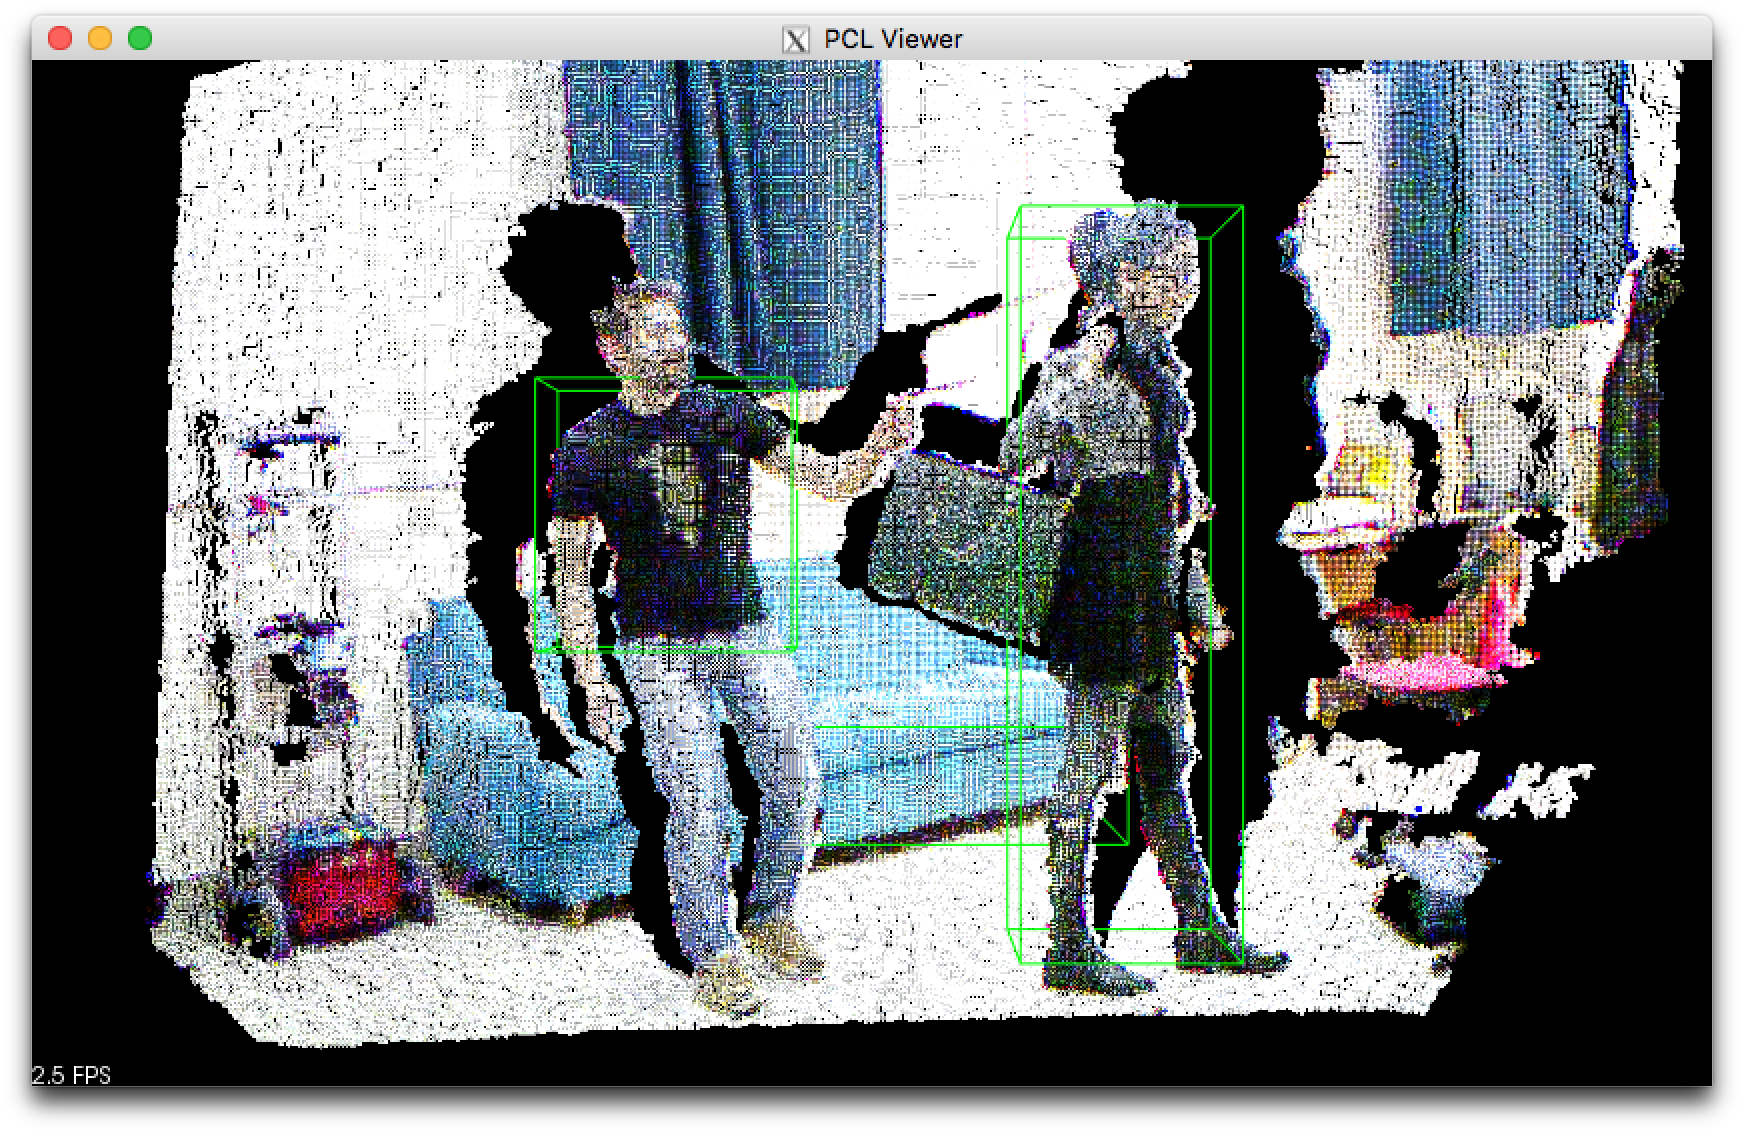
\includegraphics[scale=0.2]{good_accuracy.png}
  \caption{The figure on the right is correctly enclosed in the detection cube,
  while accuracy for the person on the left is lower}
  \label{fig:good_accuracy}
\end{figure}

\begin{figure}[h]
  \centering
  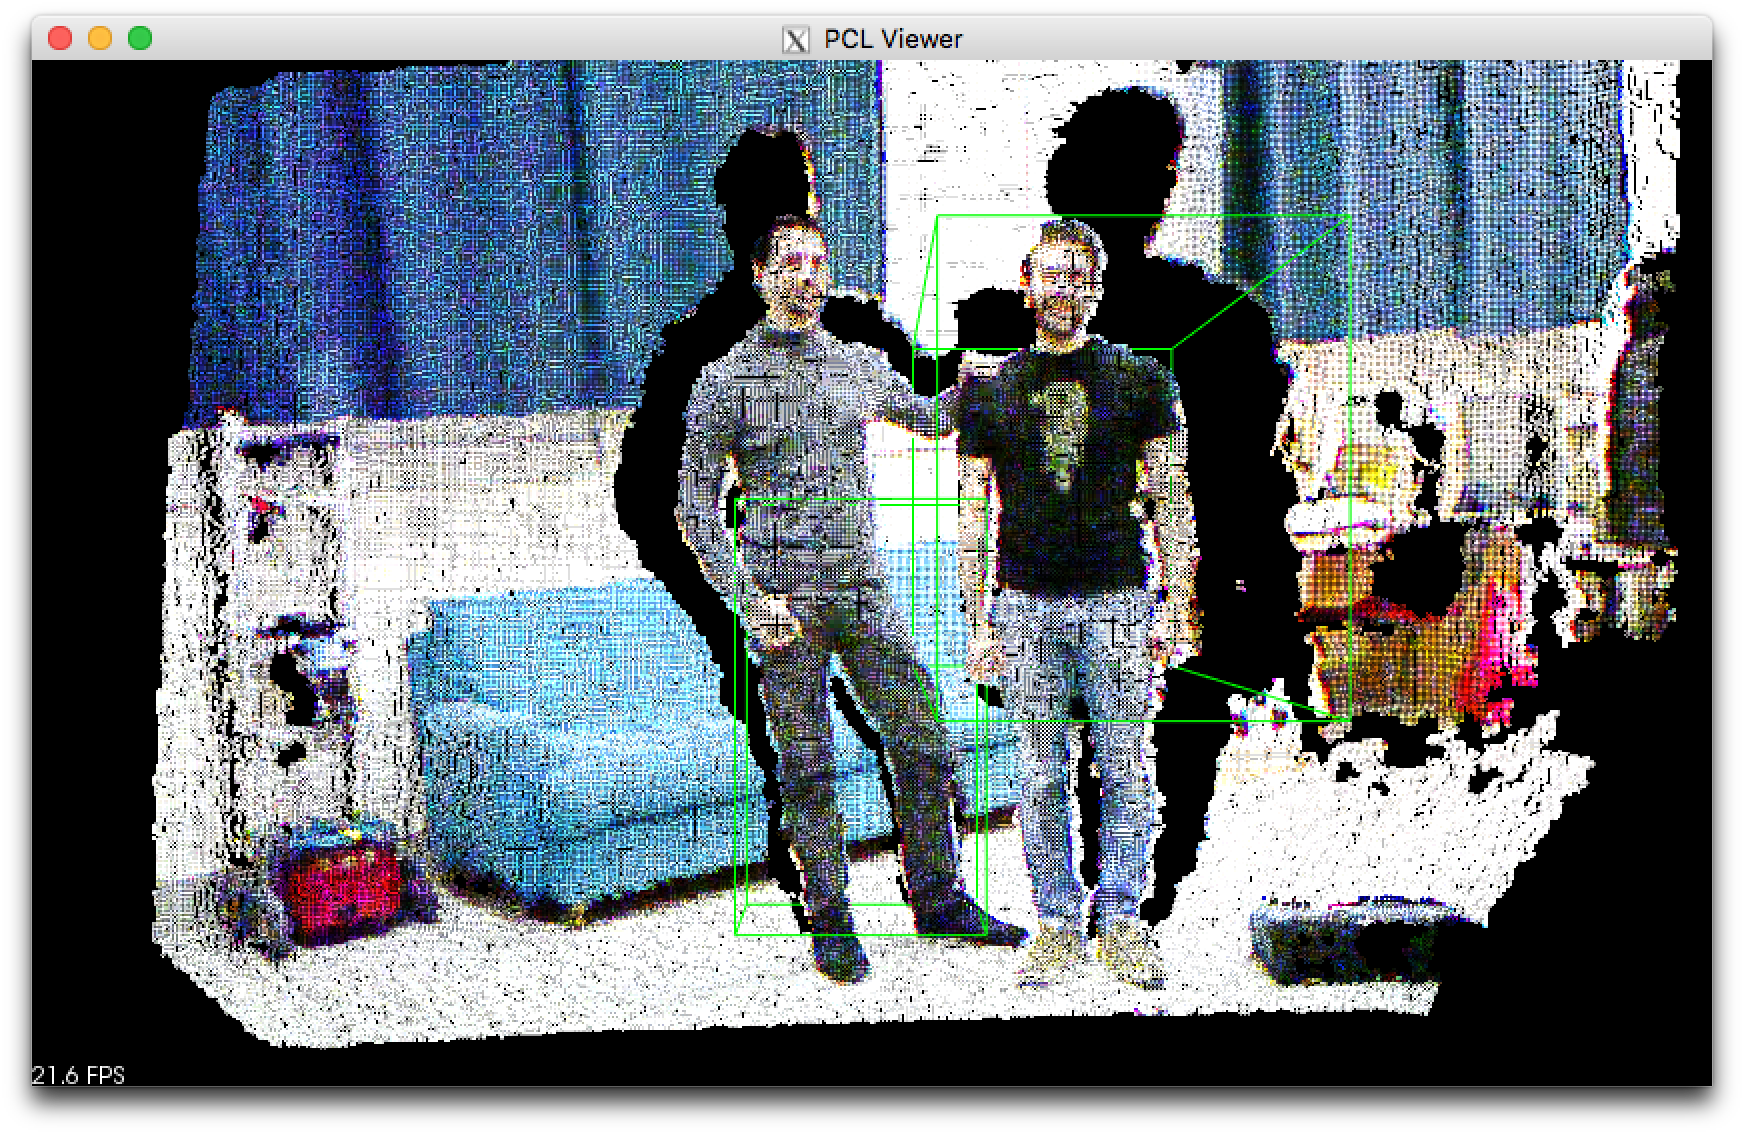
\includegraphics[scale=0.2]{good_dr_but_inaccurate.png}
  \caption{The detection on the right is oversized and excludes the lower body
  part}
  \label{fig:good_dr_but_inaccurate}
\end{figure}

A last case worth mentioning is that of multiple detections on a single person.
The case is easy to understand by simply looking at figure
\ref{fig:multiple_detections}: basically a single person is segmented with
multiple positive detections. In this case, the detected areas are
basically non-overlapping. While overall the whole person is detected, this
obviously cannot be considered accurate.

\begin{figure}[h]
  \centering
  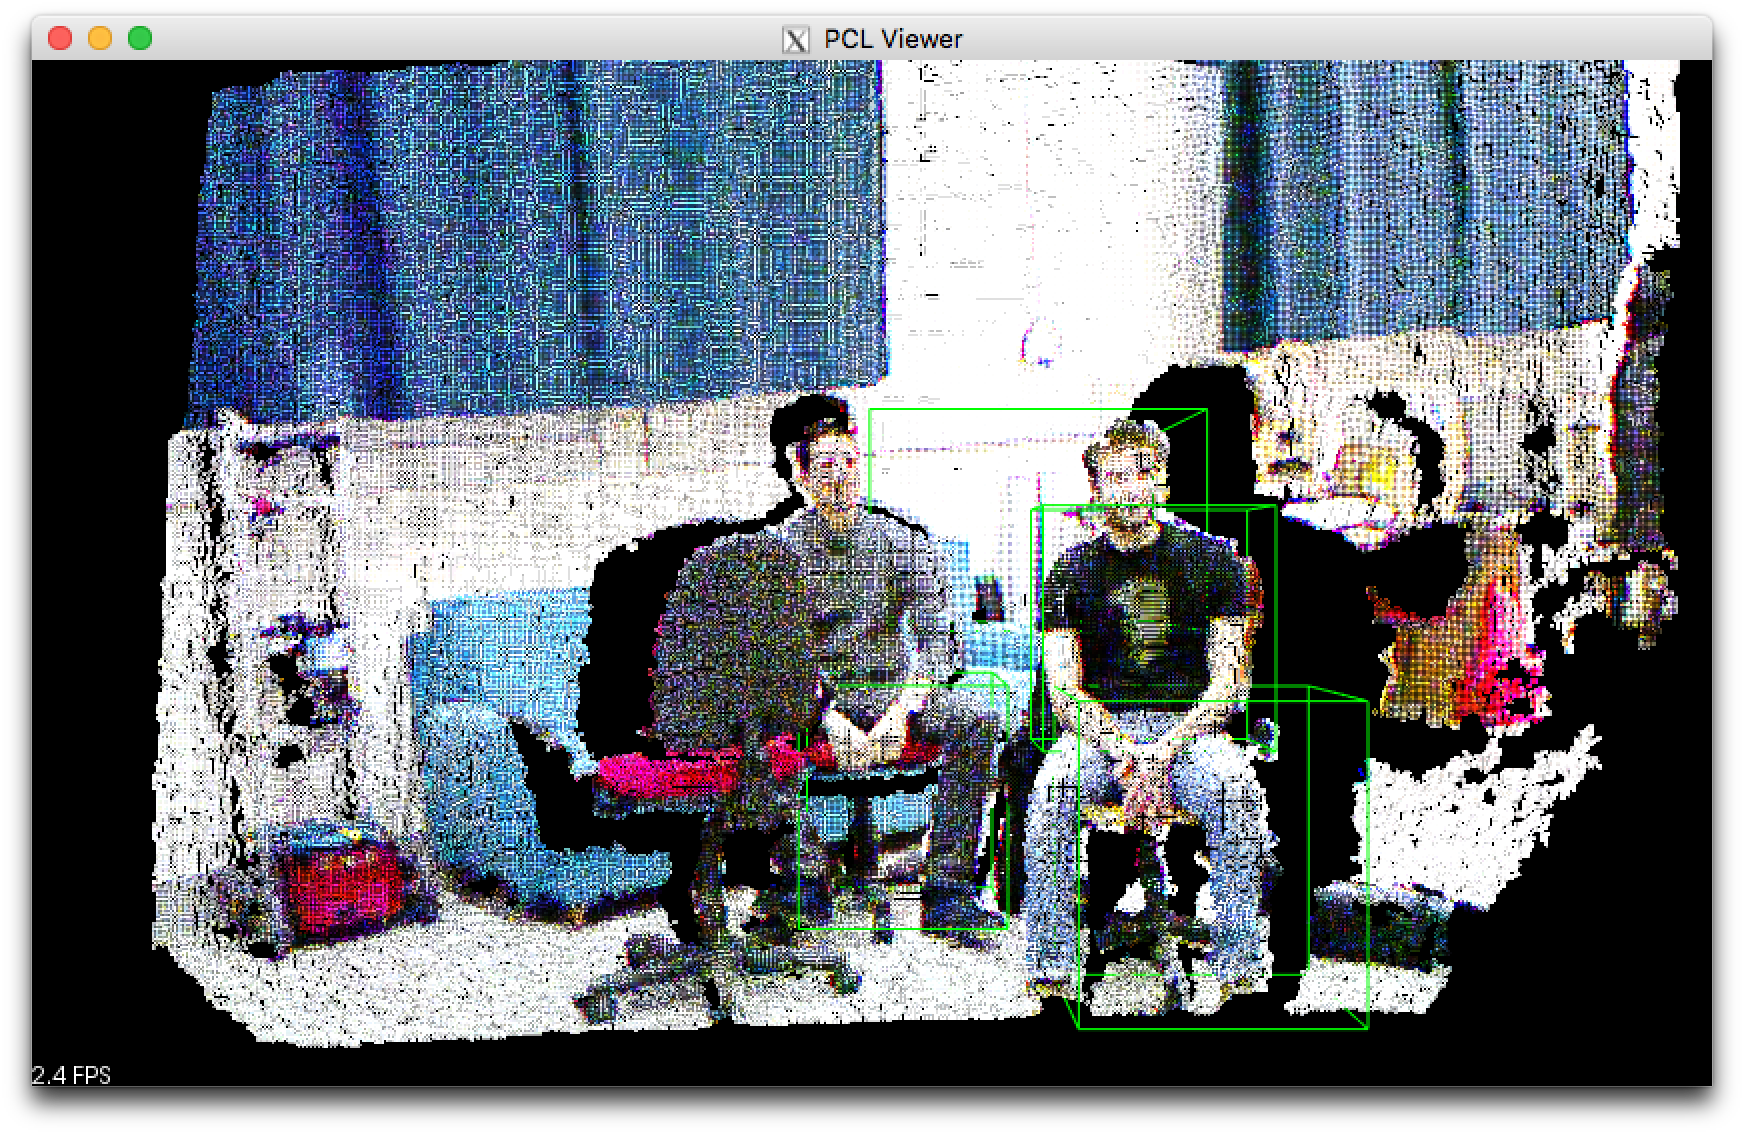
\includegraphics[scale=0.2]{multiple_detections.png}
  \caption{The person on the right is detected twice with non-overlapping
  areas}
  \label{fig:multiple_detections}
\end{figure}

Overall, detection results reflect the results that have been obtained during
the training of the detector. They don't make the algorithm "ready for
production use", but at the same time they show a clear path for performance
improvement: on one side, training the algorithm with a larger training set (and
possibly a separate validation set) is likely to give better results in term of
precision, while a more precise fine-tuning of the segmentation algorithm could
improve the algorithm's accuracy.

\subsection{Speed considerations}
All tests have been run in a virtual machine using a MacBook Pro, which hosts a
2.6 GHz Intel Core i5. Due to the significant overhead of running processes
inside a virtual machine, the numbers presented here shouldn't be considered
more in relative terms to each other rather than absolute measures of peak
performance.

Tests have been conducted to determine the algorithm's speed. Overall this is
the sum of different steps being performed. Some of these steps can be
considered as part of the core algorithm function, while others are accessory to
its practical implementation and can be excluded. For the sake of completeness
all of them have been measured.

The first measured step is opening of the scene. On the test platform this
happens on average in around 1800 ms. This step can be made faster if for
example the input is provided by a camera, thus having a continuous in-memory
stream of scenes (i.e. no disk round-trip to fetch the data).

The second measured step is the face detection on the whole scene. This runs on
average in 265 ms. As predicted, this is a very fast operation due to the low
amount of computations needed by the cascaded classifier. It's worth noting
though that the time complexity is not constant, since the more people in the
scene, the more times the classifier will have to run till the end. Also, its
speed depends on the amount of stages and features per stage; a classifier
trained with a more extended set of samples is going to be more accurate but
also slower on average.

The third measured step is the first body segmentation in a scene. This has been
measured at 60 s on average. As already discussed, since with the current
implementation the whole scene is segmented once, this step results being
extremely slow.

The fourth measured step is segmentation of a body after the first one has been
identified. This on average runs in 2 ms. As expected, this operation is very
fast since the scene has already been segmented, so at this point all left to do
is to search the cluster containing the centroid of the face that has been
identified.

The last measure is made around building the visual output of the algorithm. On
average this happens in less than 1 ms. As the first step, this is also an
accessory operation, which speed can change depending on the actual
implementation and interface requirements; nevertheless in this case its running
time is negligible with respect to the rest.

Given the analysis above, one conclusion can be drawn. In its current
incarnation, the algorithm is not suitable for real-time detection of people.
It is important to note, though, that this is not necessarily due the
algorithm's design per-se, but a few other specific components might affect this
consequence:

\begin{itemize}
  \item the actual hardware where the experiment has been run
  \item the fact that the current implementation doesn't take advantage of a
    GPU to speed up computation
  \item the fact that the current implementation is strictly sequential (i.e. it
    doesn't take advantage of any possible parallelism)
\end{itemize}

These factors are subject to change in the future and might be subject of a
development iteration aimed at improving the algorithm's overall performance.

\section{Further developments}
The results observed by developing the present paper have been useful not only to
validate the proposed approach, but also as inspiration for possible
improvements of the base technique.

An obvious improvement, achievable with what built already in this paper, is
training the detector with more samples, and possibly a more diverse set. A
fundamental principle of machine learning is that the more data is used for
training, the better the results. Also, to make the algorithm suitable for a
real-world case it's indispensible for it to be generic enough not to require
training every time a scene changes. Using a more diverse set of samples (e.g.
different scenes, different subject) would definitely be of great help.

Talking strictly about improvements over the algorithm itself instead, one first
idea is to experiment with different information when calculating features. For
example, information about a pixel's intensity could be substituted with its
depth information. The latter might prove to be a more robust information
channel rather than the former, since intensity needs normalization to account
for varying lighting conditions.

Another possible improvement is based on the observation above, and consists in
running multiple detectors in parallel and process the results with a consensus
algorithm. The different detectors can be of the same type, trained to detect
different poses (e.g. to identify profile faces rather than frontal positions);
or they could be of different types, supporting each other in case of difficult
detection (e.g. an intensity-based detector running in parallel with a
depth-based one, to compensate sensor's limitation in specific areas).

Another aspect that in this paper hasn't been considered is that of
parallelization. On a high level a cascaded detector isn't particularly suited
for a parallel implementation, but each stage could benefit from that. Since a
strong classifier requires computing a certain number of independent features
over the same scene, it's easy to imagine that calculating the feature values in
parallel would speed up the algorithm's overall performance.

A possible improvement might also lie in the use of color information: for
example, human skin lies within a specific and restricted range of colors. This
fact could be used to speed up removing negatives, so that the final cascaded
detector can be trained on more specific cases (incrementing its overall
complexity but at the same time making it more refined and precise).

Finally, one aspect that here hasn't been considered is the use of the algorithm
in a sequence of frames. It's easy to imagine how information from a
previously observed scene could help taking better decisions in subsequent
frames through subject tracking.

\bibliographystyle{plain}
\bibliography{report}

\end{document}
